\chapter{Iterators}

% NOTES: WithIndex... not needed in BSPlineDecomposition, 

% Add pointers to filters which use particular iterator types?  See alsos.

% Need to work in the concept ``multidimensional iterator'' somewhere

% Indexing

\index{Iterator!Concept}
\index{Generic Programming}
This chapter introduces the \emph{image iterator}, a fundamental and important
generic programming construct for image processing in ITK.  An iterator is a
generalization of the familiar C pointer that is used to reference data in
memory.  ITK has a wide variety of image iterators, some of which are highly
specialized to simplify common image processing tasks.

The next section is a brief introduction that defines iterators in the
context of ITK.  The programming interface common to most ITK image iterators
is decribed in section~\ref{sec:IteratorsInterface}.  Specific ITK iterator
types and examples of how they are used are documented in
sections~\ref{sec:ImageIterators}--\ref{sec:NeighborhoodIterators}.

\section{Overview}
\label{sec:IteratorsIntroduction}
% Further define iterators in the context of generic programming.
Generic programming models define functionally independent components called
\emph{containers} and \emph{algorithms}.  Container objects store data and
algorithms operate on that data.  To access data in containers, algorithms use
a third class of objects called \emph{iterators}.  An iterator is an
abstraction of a memory pointer.  Every container type must define its own
iterator type, but all iterators are written with a common interface.  This
common interface allows algorithm code to reference data in a generic way,
maintaining functional independence between algorithms and containers.

The iterator is so named because it is used for \emph{iterative}, sequential
access of container values.  Iterators appear in \code{for} and
\code{while} loop constructs, visiting each data point in turn.  A C pointer,
for example, is a type of iterator.  It can be moved forward (incremented) and
backward (decremented) through memory to sequentially reference elements of an
array. Most iterator implementations, in fact, have an interface similar to the
C pointer interface. 

% Define iterators in the context of ITK generic programming.   Differences
% between ITK iterators and other toolkits
In ITK, we use iterators to write generic image processing code for
\code{itk::Image}s instantiated with different combinations of pixel type, pixel
container type, and dimensionality.  Because ITK image iterators are
specifically designed to work with \emph{image} containers, their interface and
implementation is optimized for image processing tasks.

Writing image processing code in ITK with iterators has many specific
advantages over using the \code{itk::Image} interface directly.  Code is more
compact and often generalizes automatically to higher dimensions, algorithms
run much faster, and iterators simplify tasks such as multithreading,
neighborhood image processing, and working with non-rectilinear regions of
interest.


\section{Programming Interface}
\label{sec:IteratorsInterface}

%Creating iterators
The section describes the programming interface for ITK image iterators.  Not
all image iterators implement the full interface, and some define additional
methods.  When a specific iterator type defines any additions or restricts to this
interface, it is noted in that iterator's documentation.

\subsection{Creating Iterators}
\label{sec:CreatingIterators}
All image iterators have at least one template parameter, the image type over
which they iterate.  There is no restriction on the dimensionality of the image
or on the pixel type of the image.  Any such restrictions are imposed by the
algorithm itself, not the iterator it uses.

There are always at least two arguments to an ITK image iterator constructor.
The first argument is a smart pointer to an \code{itk::Image}.  This is the
image you want to iterate over. The second argument is an
\code{itk::ImageRegion} that specifies the \emph{iteration region}.  The
iteration region is the area of the image that the iterator will be constrained
to. It can be any sub-region of the image wholly contained in the current
\code{BufferedRegion}.  See section~\ref{sec:ImageSection} for more information
on image regions. 

Most ITK image iterators have a const and non-const version.  A non-const
iterator cannot be instantiated with a const \code{itk::Image} smart pointer.
Const versions of iterators do not allow modifying the image that they iterate
over.

Here is an example of defining and constructing an iterator using the
\code{itk::ImageRegionIterator}.  For more examples, see
sections~\ref{sec:ImageIterators}--\ref{sec:NeighborhoodIterators}.

\begin{verbatim}
typedef itk::Image<float, 3> ImageType;
typedef itk::ImageRegionConstIterator< ImageType > ConstIteratorType;
typedef itk::ImageRegionIterator< ImageType > IteratorType;

ImageType::Pointer image = SomeFilter->GetOutput();

ConstIteratorType constIterator( image, image->GetRequestedRegion() );
IteratorType iterator( image, image->GetRequestedRegion() );
\end{verbatim}


\subsection{Moving Iterators}
\label{sec:MovingIterators}
An iterator is described as \emph{walking} its iteration region.  At any time,
the iterator will reference (point to) one pixel location within that region.
Pixel locations can be thought of as N-dimensional grid indicies.  For normal,
\emph{forward iteration}, iteration runs from the beginning of the iteration
region to the end of the iteration region.  For \emph{reverse} iteration,
iteration goes from just past the end to the beginning.  There are two
corresponding starting positions for iterators, the \emph{begin} position and
the \emph{end} position.  An iterator can be moved directly to either of these
two positions using the following methods.

\begin{itemize}
\item \textbf{\code{GoToBegin()}} Points the iterator to the first valid
data element in the region.

\item \textbf{\code{GoToEnd()}} Points the iterator to \emph{one position past}
the last valid element in the region.
\end{itemize}

Note that the end position is not located within the iteration region.  This is
important to remember because attempting to dereference an iterator at its end
position will have undefined results.

%Moving iteators
ITK iterators define forward and reverse movement through their regions by
overloading the increment and decrement operators.

\begin{itemize}
\item \textbf{\code{operator++()}} Increments the iterator one position in the
positive direction.  Only the prefix increment operator is defined for ITK image
iterators.

\item \textbf{\code{operator--()}} Decrements the iterator one position in the
negative direction.  Only the prefix decrement operator is defined for ITK
image iterators. 
\end{itemize}

Figure~{\ref{fig:WalkingIterator}} illustrates typical iterator movement over
an image region.  Most iterators increment and decrement in the direction of
the fastest increasing image dimension, wrapping to the first position in the
next higher dimension at region boundaries.  In other words, this means an
iterator first moves across columns, then down rows, then from slice to slice,
etc.

\begin{figure}
\centering
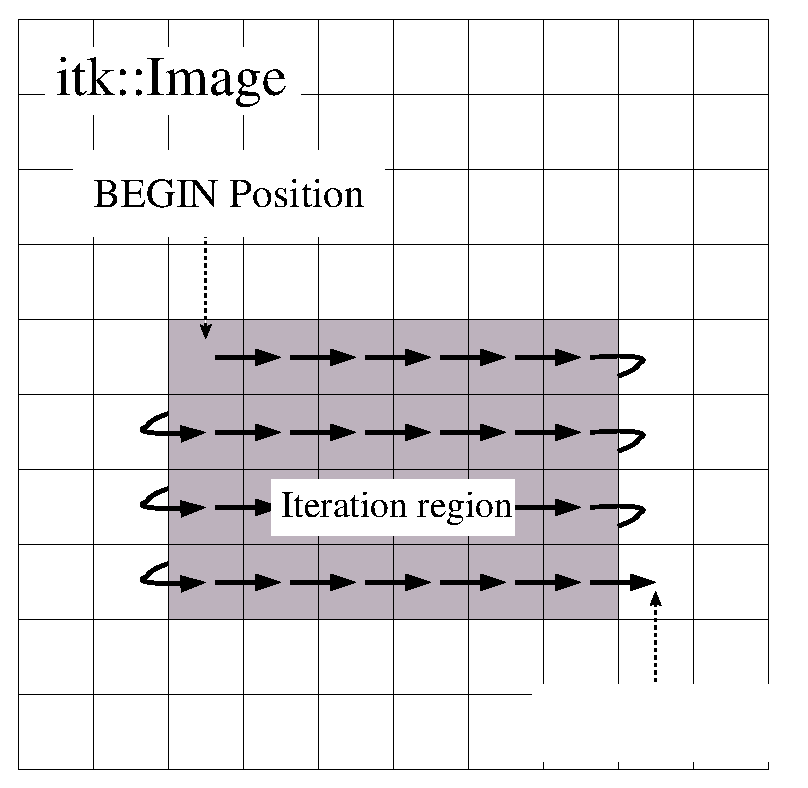
\includegraphics[width=0.4\textwidth]{IteratorFigure1.eps}
\caption[ITK image iteration]{Normal path of an iterator through an image.  The
iteration region is shown in a darker shade.  An arrow denotes a single iterator
step, the result of one \code{++} operation.}
\protect\label{fig:WalkingIterator}
\end{figure}

In addition to sequential iteration through an image, some iterators may define
random access operators.  Unlike the increment operators, random access
operators may not be optimized for speed and require some knowledge of the
dimensionality of the image and the extent of the iteration region.  

\begin{itemize}
\item \textbf{\code{operator+=( Offset )}} Moves the iterator to the pixel
position at the current index plus the specified N-dimensional \code{itk::Offset}. 

\item \textbf{\code{operator-=( Offset )}} Moves the iterator to the pixel
position at the current index minus the specified N-dimensional \code{itk::Offset}.
\end{itemize}

One final method is also defined for most iterators to move an iterator to an
absolute image index position.

\begin{itemize}
\item \textbf{\code{SetPosition( Index )}} Moves the iterator to the given
\code{itk::Index} position.
\end{itemize}

The \code{SetPosition} method may be extremely slow for more complicated
iterator types. In general, it should be used only for setting a starting
position for iteration, like you would use \code{GoToBegin()} or
\code{GoToEnd()}. 

Some iterators do not follow a predictable path through their iteration regions
and have no fixed beginning or ending pixel locations.  A conditional iterator
(section~\ref{sec:ConditionalIterators}), for example, visits pixels only if
they have certain values or connectivities.  Random iterators, increment and
decrement to random locations, and may visit a given pixel location more than
once.

%Testing for location
An iterator can be queried to determine if it has reached the end or the
beginning of its iteration region.  These methods are used as halting criteria
for iteration loops.

\begin{itemize}
\item \textbf{\code{bool IsAtEnd()}} True if the iterator points to \emph{one
position past} the end of the iteration region.

\item \textbf{\code{bool IsAtBegin()}} True if the iterator points to the first
position in the iteration region.  The method is typically used to test for the
end of reverse iteration.

\end{itemize}

An iterator can also report its current image index position.

\begin{itemize}
\item \textbf{\code{ImageIndex GetIndex()}} Returns the \code{itk::ImageIndex}
of the image pixel to which the iterator currently points.
\end{itemize}

% A note on bounds checking
For efficiency, most ITK image iterators do not perform bounds checking.  What
this means is that it is possible to move an iterator to a location outside its
valid iteration region.  Dereferencing the iterator at an out-of-bounds location
will produce an undefined result. It is left to the user to make sure the
iterator remains in bounds.  For most applications,  bounds checking is just
the standard test for \code{IsAtEnd()} or \code{IsAtBegin()} condition at each
iteration step.  Calling \code{operator+=},  \code{operator-=}, or
\code{SetPosition} on an iterator to perform random access operations may
require more careful measures. 

\subsection{Accessing Data}
\label{sec:AccessingData}
ITK image iterators define two basic methods for reading and writing pixel
values.

\begin{itemize}
\item \textbf{\code{PixelType Get()}} Returns the value of the pixel at the
iterator position.

\item \textbf{\code{void Set( PixelType )}} Sets the value of the pixel at the
iterator position.
\end{itemize}

% Describe efficiency due to inlining for all cases
The \code{Get} and \code{Set} methods are inlined and optimized for speed. In
most cases, calling either of these methods incurs no penalty over directly
dereferencing the memory pointer in the underlying image memory buffer.
\code{Get} and \code{Set} methods also support image adaptors (section~\ref{}).

There is one common case where \code{Get} and \code{Set} do incur a penalty,
however.  Consider the following code, which fetches, modifies, and then writes
a value back to the same pixel location.

\begin{verbatim}
it.Set( it.Get() + 1 );
\end{verbatim}

As written, this code requires one more memory dereference than necessary.  To
handle this case, some iterators define a third data access method.

\begin{itemize}
\item \textbf{\code{PixelType \& Value()}} Returns a reference to the pixel at
the iterator position.
\end{itemize}

The \code{Value} method can be either an lval or an rval in an expression.  It
has all the properties of \code{operator*}.  The \code{Value} method makes it
possible to rewrite our example code more efficiently.

\begin{verbatim}
it.Value()++;
\end{verbatim}

The \code{Value} method, however, cannot support the use of image adaptors.
Whenever possible, use \code{Get} and \code{Set} instead.  Because ITK filters
do not modify the contents of their input images, situations calling for
\code{Value} are less common than might be supposed.  More often than not, an
algorithm operates on two images, an input from which values are only read
(\code{Get}), and an output to which values are only written (\code{Set}).


\subsection{Iteration Loops}
\label{sec:IterationExample}
% Now give a psuedo code example for putting all of this together.
Using the methods described in the previous sections, we can now write a simple
example for pixel-wise operations in any image region.  The following code
calculates the squares all values in an input image and writes them to an
output image.

\begin{verbatim}
ConstIteratorType in(input_image,   input_image->GetRequestedRegion());
IteratorType out(output_image, input_image->GetRequestedRegion());

for (in.GoToBegin(), out.GoToBegin(); !in.IsAtEnd(); ++in, ++out)
{
  out.Set( in.Get() * in.Get() );
}
\end{verbatim}

Notice that both the input and output iterators are initialized over the same
region, the \code{RequestedRegion} of \code{input\_image}.  This is good
practice because it ensures that the output iterator walks exactly the same set
of pixel indicies as the input iterator, but does not require that the output
and input be the same size.  The only requirement here is that the output image must
contain the requested region of the input image, which will almost always be
the case when writing ITK pipeline filter objects.  Another advantage is that
only one test for the end of iteration is required in the \code{for} loop.

Equivalent code can be written to iterate through the image in reverse.
The syntax is slightly more awkward because the \emph{end} of the
iteration region is not a valid position and we can only test whether the
iterator is strictly \emph{equal} to its beginning position.  It is often more
convenient to write reverse iteration in a
\code{while} loop.

\begin{verbatim}
in.GoToEnd();
out.GoToEnd();
while ( ! in.IsAtBegin() )
{
  --in;
  --out;
  out.Set( in.Get() * in.Get() );
}

\end{verbatim}
% Need a paragraph or two about other image methods like GetIndex(), etc.  Are
%these universally defined?

%\begin{itemize}
%\item \textbf{\code{index GetIndex()}} 
%\item \textbf{\code{SetIndex(index)}}
%\end{itemize}

%\begin{itemize}
%\item \textbf{\code{operator==}}
%\item \textbf{\code{operator<}} 
%\item \textbf{\code{operator<=}}
%\item \textbf{\code{operator>}}
%\item \textbf{\code{operator>=}}
%\end{itemize}

%operator +=, -=, etc

% SetIndex()

% operator <, operator >, etc.


\section{Image Iterators}
\label{sec:ImageIterators}
%Introduction and overview
This section describes iterators that walk rectilinear regions in images and
reference a single pixel.  The \code{itk::ImageRegionIterator} is the basic,
general purpose ITK image iterator.  The rest of the
iterators described in this section are variations on
\code{itk::ImageRegionIterator} and incorporate specializations designed to 
speed up or encapsulate common tasks.

% Each of the iterators has a const and non-const version

\subsection{itk::ImageRegionIterator}
\label{sec:itkImageRegionIterator}
\input{ImageRegionIterator.tex}

\subsection{itk::ImageRegionIteratorWithIndex}
\label{sec:itkImageRegionIteratorWithIndex}
\input{ImageRegionIteratorWithIndex.tex}

\subsection{itk::ImageLinearIteratorWithIndex}
\label{sec:itkImageLinearIteratorWithIndex}
\input{ImageLinearIteratorWithIndex.tex}

\subsection{itk::ImageSliceIteratorWithIndex}
\label{sec:itkImageSliceIteratorWithIndex}
\input{ImageSliceIteratorWithIndex.tex}

\subsection{itk::ImageRandomConstIteratorWithIndex}
\label{sec:itkImageRandomConstIteratorWithIndex}
\input{ImageRandomConstIteratorWithIndex}


\section{Conditional Iterators}
\label{sec:ConditionalIterators}
This section describes iterators that walk only pixels in an image region whose
values satisfy a specified condition.  The condition is usually based on some
function of the image values, such as comparing to a threshold.  When the
condition function returns \code{true} at a pixel location, the iterator
includes that location in its path.  The biggest use of these iterators is for
walking non-rectilinear regions of interest, such as might be defined by
implicit geometric shape functions or connected component regions.

%./Common/itkConditionalConstIterator.h (BaseClass)
%./Common/itkConditionalIterator.h (BaseClass)
%./Common/itkFloodFilledFunctionConditionalConstIterator.h (BaseClass)
%./Common/itkFloodFilledFunctionConditionalIterator.h (BaseClass)

%[ here are all classes where these filters are used:
% ./BasicFilters/itkConfidenceConnectedImageFilter.txx (ImageFunction)
% ./BasicFilters/itkConnectedThresholdImageFilter.txx (ImageFunction)
% ./BasicFilters/itkIsolatedConnectedImageFilter.txx (ImageFunction)
% ./BasicFilters/itkNeighborhoodConnectedImageFilter.txx (ImageFunction)
%
% ./Common/itkBinaryBallStructuringElement.txx (SpatialFunction)
% ./Common/itkBloxCoreAtomImage.txx (SpatialFunction)
% ./BasicFilters/itkBloxBoundaryPointToCoreAtomImageFilter.txx (SpatialFunction)
% ./BasicFilters/itkBloxBoundaryPointImageToBloxBoundaryProfileImageFilter.txx (SpatialFunction)
%]

\subsection{itk::FloodFilledImageFunctionConditionalIterator}
\label{itk::FloodFilledImageFunctionConditionalIterator}
%./Common/itkFloodFilledImageFunctionConditionalConstIterator.h
%./Common/itkFloodFilledImageFunctionConditionalIterator.h


\subsection{itk::FloodFilledSpatialFunctionConditionalIterator}
\label{itk::FloodFilledSpatialFunctionConditionalIterator}
%./Common/itkFloodFilledSpatialFunctionConditionalConstIterator.h
%./Common/itkFloodFilledSpatialFunctionConditionalIterator.h


\section{Neighborhood Iterators}
\label{sec:NeighborhoodIterators}
This section describes the ITK image iterators designed for working with
neighborhoods of image pixels in an image. 
% -Designed to encapsulate common neighborhood management functionailty
% -efficiently manage access to entire N-dimensional neighborhoods, making
% localized image processing algorithms simple to write and to generalize to
% higher dimensions. 
% - walk rectilinear regions
% 

%Do not support image adaptors

%[Be sure to reference Section: Neighborhood Filters]

% Describe the common interface and other redefined methods

\subsection{itk::NeighborhoodIterator}
\label{sec:itkNeighborhoodIterator}

% \input{NeighborhoodIterator1.tex}
%./Common/itkConstNeighborhoodIterator.h
%./Common/itkNeighborhoodIterator.h

% Example: derivative
% Example: convolution filtering
% Example: boundary conditions
% Example: walking faces



\subsection{itk::ShapedNeighborhoodIterator}
\label{sec:itkShapedNeighborhoodIterator}
./Common/itkConstShapedNeighborhoodIterator.h
./Common/itkShapedNeighborhoodIterator.h


% ADD A SECTION WITH TIPS, SUGGESTIONS ON USING ITERATORS?  EXTENDING ITERATORS?
% USING ITERATORS FOR MULTITHREADING EXAMPLE?
